%\documentclass[10pt,twocolumn,letterpaper,draft]{article}
\documentclass[10pt,letterpaper]{ctexart}

\usepackage{cvpr}
% \usepackage{epsfig}
\usepackage{graphicx}
\usepackage{amsmath}
\usepackage{amssymb}
% \usepackage{color}
\usepackage{subfigure}
\usepackage{algorithm}
\usepackage{algorithmicx}
\usepackage{algpseudocode}
\usepackage{listings}

\lstset{language=C++,
    basicstyle=\ttfamily,
    frame=single,
    keywordstyle=\color{blue}\ttfamily,
    stringstyle=\color{magenta}\ttfamily,
    commentstyle=\color{green}\ttfamily,
    morecomment=[l][\color{magenta}]{\#},
    morekeywords={*,uint_fast64_t}
}

\renewcommand{\labelenumi}{\alph{enumi}.} % Make numbering in the enumerate environment by letter rather than number (e.g. section 6)
\floatname{algorithm}{算法}
\renewcommand{\algorithmicrequire}{\textbf{输入:}}
\renewcommand{\algorithmicensure}{\textbf{输出:}}
\renewcommand{\lstlistingname}{代码清单}

\usepackage{enumitem}
\setenumerate[1]{itemsep=0pt,partopsep=0pt,parsep=\parskip,topsep=5pt}
\setitemize[1]{itemsep=0pt,partopsep=0pt,parsep=\parskip,topsep=5pt}
\setdescription{itemsep=0pt,partopsep=0pt,parsep=\parskip,topsep=5pt}

% Include other packages here, before hyperref.

% If you comment hyperref and then uncomment it, you should delete
% egpaper.aux before re-running latex.  (Or just hit 'q' on the first latex
% run, let it finish, and you should be clear).
\usepackage[pagebackref=true,breaklinks=true,letterpaper=true,colorlinks,bookmarks=false]{hyperref}


\cvprfinalcopy % *** Uncomment this line for the final submission

\def\cvprPaperID{159} % *** Enter the CVPR Paper ID here
\def\httilde{\mbox{\tt\raisebox{-.5ex}{\symbol{126}}}}

\newcommand{\mypara}[1]{\paragraph{#1.}}

\graphicspath{{figures/}}

% Pages are numbered in submission mode, and unnumbered in camera-ready
%\ifcvprfinal\pagestyle{empty}\fi
\setcounter{page}{1}


%\begin{CJK*}{GBK}{song}

\newcommand{\figref}[1]{图\ref{#1}}
\newcommand{\tabref}[1]{表\ref{#1}}
\newcommand{\equref}[1]{式\ref{#1}}
\newcommand{\secref}[1]{第\ref{#1}节}

\ctexset{
  section={
          name={,、},
          number={\chinese{section}},
          format={\heiti},
          beforeskip={0.1ex},
          afterskip={0.1ex},
          aftername={\nobreak},
          indent={\parindent},
          },
}
\usepackage{zhnumber}

\newcommand\zhsubsec[1]{{% 中文小节
\bfseries{
\stepcounter{subsection}(\zhnum{subsection}){#1}}
\vspace{0.1pt}%
}}

%%%%%%%%% TITLE
\begin{document}
\pagestyle{plain}
\title{
    \begin{center}
        \phantom{Start!}
    	  \vspace{2cm}
        \center{\zihao{1} 中山大学数据科学与计算机学院}
        \center{\zihao{2} 《高性能程序设计基础》实验6}
        \center{(2018-2019学年秋季学期)}
    \end{center}
}
\maketitle

\begin{center}
    \setlength{\baselineskip}{40pt}
    \vspace{1cm}
    \zihao{-2}
    \center{
        \begin{tabular}{cc}
      	学\qquad 号:& \underline{~~~~~~16337113~~~~~~}  \\
      	姓\qquad 名:& \underline{~~~~~~~劳马东~~~~~~~}  \\
        教学班级:   & \underline{~~~~~教务2班~~~~~}  \\
      	专\qquad 业:& \underline{~~~~~~~~~超算~~~~~~~~}  \\
      	\end{tabular}
    }
\end{center}
\pagebreak

%%%%%%%%% BODY TEXT %%%%%%%%%%%%
% \begin{enumerate}[itemindent=2.5em,label=\arabic*、]
% \end{enumerate}

% \begin{algorithm}
%     \begin{algorithmic}[1] %每行显示行号
%         \Function {$TreeSearch$}{$Frontier, Successors,
%         \EndFunction
%     \end{algorithmic}
% \end{algorithm}

% \begin{figure}[h]
%   \centering
%   \subfigure[Completeness]{
%   \includegraphics[width=0.4\textwidth]{dfs-1.png}
%   \label{fig:dfs-1}}
% \end{figure}

\section{实验题目}
\begin{enumerate}[itemindent=1.5em,label=\arabic*、]
\item 完成正则采样排序PSRS的MPI算法;
\item 按要求使用MPI集合通信。
\end{enumerate}

\section{正则采样排序概述}
快速排序算法的效率相对较高,并行算法在理想的情况下时间复杂度可达到$O(n)$,但它有一个严重的问题:
会造成严重的负载不平衡,最差情况下算法的复杂度可达$O(n^2)$。并行正则采样排序克服了这一缺点,
是一种基于均匀划分的负载平衡的并行排序算法。

\zhsubsec{算法流程}

\begin{figure}[H]
  \centering
  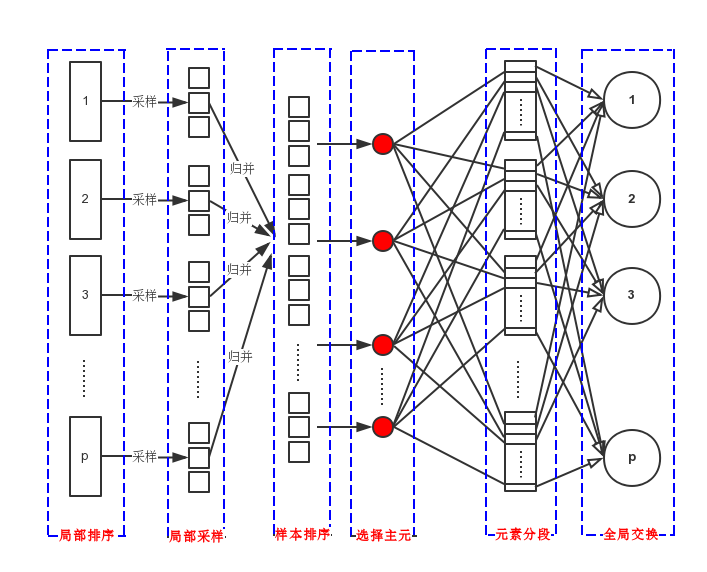
\includegraphics[width=0.7\textwidth]{steps.png}
  \label{fig:steps}
  \caption{正则采样排序示意图}
\end{figure}

\par 假设待排序的元素n个,处理器p个,算法大体流程如下。
\begin{enumerate}[itemindent=3em,label=\arabic*、]
  \item 首先将这n个元素均匀的分成p部分,每部分包含$\frac{n}{p}$个元素(如图1矩形)。每个处理器负责其中的一部分,并对其进行局部排序;
  \item 为确定局部有序序列在整个序列中的位置,每个处理器从各自的局部有序序列中选取几个代表元素(如图1第一列正方形);
  \item 将这些代表元素进行排序后选出p-1个主元(如图1红色圆形);
  \item 每个处理器根据这p-1个主元将自己的局部有序序列分成p段;
  \item 然后通过全局交换的方式,将p段有序序列分发给对应的处理器(如图1大圆),使第i个处理器都拥有各个处理器的第i段,
  共p段有序序列。
  \item 每个处理器对这p段有序序列进行排序。最后,将各个处理器的有序段按顺序汇合起来,就是全局有序序列了。
\end{enumerate}

\section{实验过程}
\zhsubsec{元素划分与采样}

出于方便和性能考虑,每个进程直接从文件中并行读取元素。并行读取最重要的是解决文件指针
定位的问题,即每个进程该从什么位置开始读取多少个元素?假设$p$个进程分别编号为$0、1...p-2、p-1$,
则显然进程$i$开始读的位置是前$i-1$个进程所读元素的和,即:
\begin{equation}
  f(i) =
    \begin{cases}
      f(i-1) + balance(i-1) & i=1, 2, ..., p-2, p-1\\
      0 & i=0
    \end{cases}
\end{equation}
其中$balance$函数返回对应进程的负载,即读取多少个元素。
\par 那么如何相对均衡地分配负载呢?方法是先给每个进程分配$\lfloor\frac{n}{p}\rfloor$
个元素,然后将剩下的$r$个元素分配给编号$0$到$r-1$的进程。
\begin{lstlisting}[caption=并行读取元素,label={code:read},captionpos=b]
vector<uint_fast64_t> divide_read_directly(istream& in, 
                                            uint_fast64_t n, 
                                            MPI_Comm comm) 
{
    Comm_Info info(comm);
    // 获取每个进程对应的负载(均衡)
    vector<uint_fast64_t> balance = get_v<uint_fast64_t>(n, info.comm_size);
    // 得到自己的负载的元素个数
    uint_fast64_t my_balance = balance[info.rank];
    vector<uint_fast64_t> local(my_balance);
    // 计算负载的前缀和,每个数代表对应进程开始读的位置
    vector<uint_fast64_t> prefixes = get_prefix_sum<uint_fast64_t>(balance);
    // 每个数8个字节,指针定位时乘上8(加1是为了跳过开头表示元素总数的那个数)
    in.seekg((prefixes[info.rank] + 1) * 8, ios::beg);
    for (auto& x: local)
        read(in, x);
    return local;
}
\end{lstlisting}

\begin{enumerate}[itemindent=4em,label=\arabic*、]
\item 本地数据排序
\par \qquad 排序原则上采用任何排序算法都可以,但是由于数据量比较大,如果使用空间复杂度
较大的算法(如快速排序和归并排序),就很容易超出内存限制,导致程序崩溃。因此,实验中使用
了STL的stable\_sort,它使用桶排序算法对序列原地排序,并且时间复杂度是$O(n \log n)$。
\item 按进程数p等间隔采样
\par \qquad 每个进程从其局部有序序列中选取$p$个样本,因此总共有$p^2$个样本,取数间隔为$\frac{n}{p^2}$。
\begin{lstlisting}[caption=排序与采样,label={code:local_sample},captionpos=b]
stable_sort(local.begin(), local.end());
  
int num_samples = info.comm_size * info.comm_size;
vector<uint_fast64_t> sample = copy_every_n(local, n / num_samples);
\end{lstlisting}

\end{enumerate}

\zhsubsec{划分主元}
\begin{enumerate}[itemindent=2.5em,label=\arabic*、]
\item 收集样本:一个进程(0号)用MPI\_Gatherv收集样本并对所有样本进行排序;
\item 采样获得主元:按进程数p对全体样本等间隔采样;
\item 用MPI\_Bcast广播主元。
\end{enumerate}

\begin{lstlisting}[caption=划分主元并广播,captionpos=b]
vector<uint_fast64_t> global_sample;    // 存储全部样本
// 收集每个进程的样本
Gather(sample, global_sample, MPI_UINT64_T, 0, MPI_COMM_WORLD);
// 存储主元,p-1个
vector<uint_fast64_t> pivots(info.comm_size - 1);
if (info.rank == 0) {
    // 对所有样本排序,使用归并排序
    auto it = global_sample.begin();
    for (int j = 0; j < info.comm_size - 1; ++j) {
        it += info.comm_size;
        inplace_merge(global_sample.begin(), it, it + info.comm_size);
    }
    
    // 从第p个开始,等间隔p采样主元,最终采得p-1个
    pivots = copy_every_n(global_sample, info.comm_size, info.comm_size);
}
// 广播主元
Bcast(pivots, MPI_UINT64_T, 0, MPI_COMM_WORLD);
\end{lstlisting}

\zhsubsec{交换数据}
\begin{enumerate}[itemindent=2.5em,label=\arabic*、]
\item 本地数据分块
\par \qquad 将有序数组a中的元素,以数组d中的元素为分界线,划分成多个段。算法首先变量d中的每个分界点x,将小于
或等于x的元素存储在一维数组seg中,这个seg数组就是一段,最终所有的seg数组组成一个二维数组。
\newpage
\begin{lstlisting}[caption=数组分段,captionpos=b]
template <typename T>
vector<vector<T>> divide_seg(const vector<T>& a, const vector<T>& d) {
    vector<vector<T>> res;
    auto it = a.begin();
    for (T x: d) {
        vector<T> seg;
        while (it != a.end() && *it <= x) {
            seg.push_back(*it);
            ++it;
        }
        res.push_back(seg);
    }
    // 处理最后由于it==a.end()退出的情况
    res.push_back(vector<T>(it, a.end()));
    return res;
}
\end{lstlisting}

\item 全交互
\par \qquad 该过程每个进程将自己局部序列的p个段按顺序发给p个进程,使用一个循环来
将p个段Gather给对应进程,并返回各个进程第i段的长度,用数组seg\_length记录,它的作用
是在之后的归并排序中计算每个有序子段的范围。
\begin{lstlisting}[caption=全交互,captionpos=b]
vector<vector<uint_fast64_t>> local_blocks = divide(local, pivots);
// 存储全交互结果
vector<uint_fast64_t> local2;
// 存储从各个进程收到的段长度
vector<int> seg_length;
for (int i = 0; i < info.comm_size; ++i) {
    // 向进程i聚集段i,并返回从各个进程收到的元素个数(段长度)
    vector<int> tmp = Gatherv(local_blocks[i], local2, MPI_UINT64_T, 
                              i, MPI_COMM_WORLD);
    if (info.rank == i)
        seg_length = tmp;
}
\end{lstlisting}
\end{enumerate}

\zhsubsec{归并排序}
\par 由于从各个进程收集到的子序列都是有序的,因此可以充分利用这一特性进行归并排序,而不是对整个序列应用
其他排序算法。此外,为了降低空间复杂度,使用STL的原地归并算法,而不是普通归并(利用第三个数组存储
归并中间结果)。
\newpage
\begin{lstlisting}[caption=有序子段归并,captionpos=b]
auto it = local2.begin();
for (int j = 0; j < info.comm_size - 1; ++j) {
    it += seg_length[j];
    inplace_merge(local2.begin(), it, it + seg_length[j + 1]);
}
\end{lstlisting}

\section{实验结果及分析}


\end{document}
